% !TEX program = xelatex
% ============================================================
%  财富庄园 · Wealth Manor —— 企划书（合并版）
%  合并来源：财富庄园3.docx（一/二章）、个人理财系统企划书（三章）、财富庄园C.docx（四/五/六章）
%  编译：latexmk -xelatex 合并版.tex
% ============================================================
\documentclass[12pt,a4paper]{ctexart}

% ---------- 宏包 ----------
\usepackage[margin=2.4cm,top=2.8cm,bottom=2.8cm]{geometry}
\usepackage{amsmath}
\usepackage{graphicx}
\usepackage{booktabs}
\usepackage[table]{xcolor}
\usepackage{array}
\usepackage{longtable}
\usepackage{tikz}
\usetikzlibrary{positioning,arrows.meta,shadows,calc}
\usepackage{enumitem}
\usepackage{fancyhdr}
\usepackage{hyperref}
\usepackage{float}
\usepackage{caption}

% ---------- 颜色 ----------
\definecolor{icbcred}{HTML}{007AFF}
\definecolor{manorgreen}{HTML}{34C759}
\definecolor{rowgray}{HTML}{F5F5F5}

% ---------- 页眉页脚 ----------
\pagestyle{fancy}
\fancyhf{}
\fancyhead[C]{\small\color{icbcred}财富庄园·Wealth Manor —— 企划书}
\fancyfoot[C]{\small\thepage}
\renewcommand{\headrulewidth}{0.4pt}

% ---------- 超链接样式 ----------
\hypersetup{
  colorlinks=true,
  linkcolor=icbcred,
  urlcolor=manorgreen,
  pdftitle={财富庄园企划书（合并版）},
  pdfauthor={财富庄园团队}
}

% ---------- 表格行着色 ----------
\rowcolors{2}{rowgray}{white}

% ---------- 列表与段落间距 ----------
\setlist{itemsep=2pt,topsep=3pt}
\linespread{1.25}
\setcounter{tocdepth}{2}

% ---------- 自定义命令 ----------
% 一级/二级标题（手动编号，与目录大纲一致）
\newcommand{\ch}[1]{\section*{#1}\addcontentsline{toc}{section}{#1}}
\newcommand{\sect}[1]{\subsection*{#1}\addcontentsline{toc}{subsection}{#1}}
% 三级小标题（不进目录）
\newcommand{\sub}[1]{\subsubsection*{#1}}
% 加粗引语段落
\newcommand{\lead}[2]{\noindent\textbf{#1}#2\par\vspace{0.6em}}

\begin{document}

% ============================================================
% 封面
% ============================================================
\begin{titlepage}
\centering
\vspace*{2.2cm}

{\color{icbcred}\rule{\textwidth}{2pt}}\\[0.6cm]
{\Huge\bfseries 财富庄园 · Wealth Manor}\\[0.5cm]
{\LARGE 游戏化智能财富管理与金融素养教育平台}\\[0.3cm]
{\color{icbcred}\rule{\textwidth}{2pt}}\\[1.8cm]

{\Large\bfseries 企 \quad 划 \quad 书}\\[2.6cm]

\begin{tabular}{rl}
\textbf{参赛方向} & 财富管理服务 · 普惠金融\\
\textbf{团队成员} & 王思佳 \quad 阮馨莹 \quad 张煜杰\\
\end{tabular}

\vfill
{\large 2026年8月}
\end{titlepage}

% ============================================================
% 目录
% ============================================================
\tableofcontents
\newpage

% ============================================================
% 一、执行摘要（来源：财富庄园3.docx 第1章）
% ============================================================
\ch{一、执行摘要}

\sect{（一）项目背景}
\lead{1. 居民财富管理需求持续增长。}{随着我国居民财富水平不断提升，居民金融需求正在由传统的单一储蓄需求逐步向资产配置、风险管理和长期财富规划转变。截至2025年末，我国银行理财市场存续规模达到33.29万亿元，较年初增长11.15\%；持有理财产品的投资者数量达到1.43亿个，其中个人投资者占比98.64\%。与此同时，居民财富管理的关注重点也正在发生变化。过去，用户更多关注"购买什么金融产品"，而随着存款、基金、理财、证券、保险、房产等资产类型不断丰富，用户开始进一步关注自身整体财富状况以及不同资产之间的配置关系。财富管理正在从"选择一个产品"逐渐转向"管理全部财富"。然而，财富管理需求增长与财富管理能力提升之间仍存在一定差距。许多用户能够看到自己的某一个账户或某一项资产，却难以从整体角度理解自己的资产结构、收益变化、风险水平和长期财富目标。因此，财富管理服务需要进一步从"提供金融产品"向"帮助用户看懂、管理和规划整体财富"转变。}
\lead{2. 数字化财富管理成为年轻用户的新需求。}{18--35岁年轻群体正处于财富管理习惯形成的重要阶段。大学生、初入职场者和青年家庭正在经历第一次获得稳定收入、第一次独立管理资金、第一次进行投资，以及第一次承担购房、家庭和养老等长期财富责任。与此同时，年轻用户高度熟悉移动APP、游戏、社交和人工智能等数字化交互方式。相比传统的宣传手册、线下讲座和单向课程，年轻用户更加习惯通过互动、可视化和场景化方式获取信息。因此，面向年轻群体的财富管理服务不仅需要提供金融产品，更需要建立一个能够让用户愿意参与、容易理解、持续使用的数字化财富管理场景。财富庄园正是在这一背景下提出。}

\sect{（二）行业痛点}
\lead{1. 财富信息分散，"有资产"但"看不清财富"。}{当前居民财富结构日益复杂，用户可能同时拥有银行存款、理财、基金、证券、保险、房产等多种资产，而这些资产往往分散在不同账户和机构中。用户能够看到单个账户，却难以形成完整的个人财富版图。这使得用户在进行财富管理时容易陷入"只看单个产品、不看整体资产"的状态，也难以判断自身的资产配置是否合理。因此，行业需要一种能够将分散财富信息进行整合，并以更加直观方式呈现个人整体财富状况的服务工具。}
\lead{2. 金融知识与实际财富管理行为存在断层。}{当前金融机构已经开展大量金融知识普及和投资者教育服务，但用户"知道"和"做到"之间仍存在明显距离。2025年消费者金融素养调查显示，我国消费者金融素养指数为67.61，其中金融知识得分为76.25，而金融行为得分仅为54.28，金融行为得分明显低于金融知识水平。这说明当前金融教育面临的核心问题已经不只是"用户不知道金融知识"，而是用户即使理解风险、收益、分散配置和长期投资等概念，也不一定能够将其转化为持续的财富管理行为。因此，行业需要从单纯的知识传播进一步转向行为引导和长期陪伴。}
\lead{3. 金融产品丰富，但年轻用户理解成本较高。}{当前银行可以提供存款、理财、基金、保险、贵金属、外汇等多元化金融服务，但产品种类增加并不意味着用户理解成本降低。对于财富管理经验有限的年轻用户而言，他们往往难以快速理解不同金融产品之间的风险、收益、期限和流动性差异，也难以判断某项产品是否与自身财富目标相匹配。因此，银行需要进一步降低财富管理的专业门槛，将复杂的金融概念转化为更加直观、易理解的表达方式。}
\lead{4. 传统财富管理缺少持续、互动的陪伴场景。}{传统金融服务往往在用户产生明确金融需求后发生，例如有存款需求时办理存款、有投资需求时购买理财。但真正的财富管理是一个长期过程。从第一次获得收入，到第一次储蓄、第一次投资，再到购房、组建家庭和养老，每一个人生阶段都会产生新的财富管理需求。因此，银行需要从"用户有需求之后提供产品"进一步转向"从用户开始管理财富时就持续陪伴"。财富庄园希望通过游戏化交互、财富可视化和AI辅助，将财富管理融入用户日常使用场景。}

\sect{（三）项目总览}
\lead{1. 项目定位。}{基于上述行业痛点，项目提出"财富庄园（Wealth Manor）"——一款新型游戏化智能财富管理与金融素养教育平台。项目以"庄园经营"为核心交互载体，将现实财富管理中的资产、收益、市场变化、理财行为和财富目标转化为可视化、可互动的游戏机制。财富庄园不是将金融与游戏简单叠加，而是以真实财富数据为基础，将游戏作为用户理解和参与财富管理的交互入口。其核心理念为：游戏降低门槛，财富树呈现全局，AI辅助决策，教育培养能力，长期陪伴财富成长。平台最终形成：真实财富 $\rightarrow$ 游戏化呈现 $\rightarrow$ 智能分析 $\rightarrow$ 行为反馈 $\rightarrow$ 财富成长的服务闭环。}
\lead{2. 核心产品结构。}{财富庄园采用"模拟器核心 + 专项训练 + 成长陪伴"三层游戏结构。第一层\textbf{财富人生模拟器（核心玩法）}：回合制家庭财富现金流经营——每一种金融产品都是一张"英雄卡"，完整呈现风险、收益、流动性、法律与合规、税收、到期日、特殊情况七维属性；用户完成风险评估后获得初始可购阵容（对应游戏中的英雄池），在给定收入与财富水平下按月经营，经历经济周期与政策变化，最终在特定时间点满足购房、教育、养老等现金流目标，并通过"财富偏差护照"复盘冲动消费、流动性不足、集中度过高与错过政策窗口四类偏差。第二层\textbf{专项理财小游戏}：3--5分钟一局的预算管理、金融反诈、资产配置与投资情绪训练。第三层\textbf{财富庄园（长期成长陪伴层）}：将学习成果、行为变化与财富规划转化为种植、天气、任务等长期可视化成长，AI财富助手与全资产看板贯穿全程。}
\lead{3. 核心产品逻辑。}{财富庄园围绕"真实财富"建立游戏化交互。用户进入庄园后，可以通过财富树了解自身整体财富版图；通过资产看板查看不同资产的结构和变化；通过天气了解市场环境；通过植物成长感受不同资产的收益变化；通过AI助手进一步理解资产风险和配置情况；通过任务和知识问答逐渐建立财富管理习惯。因此，游戏在财富庄园中并非单纯的娱乐功能，而是承担金融信息可视化、用户行为反馈和财富教育交互的作用。平台通过这一方式将原本抽象的财富数据转化为用户能够理解和持续关注的"财富成长过程"。}

\noindent\textbf{总结：}财富庄园不是把理财变成游戏，而是用游戏作为财富管理的交互入口，让真实财富可视化、让金融知识可理解、让财富行为可反馈，让银行成为用户长期财富成长的陪伴者。

\sect{（四）社会价值}
\lead{1. 提升居民金融素养。}{财富庄园通过游戏化方式降低金融知识学习门槛，将风险、收益、资产配置、长期投资和复利等抽象概念转化为植物成长、市场天气和财富树变化等具体体验，使金融教育从单纯的"告诉用户应该怎么做"，进一步转向"让用户理解为什么这样做"。}
\lead{2. 推动金融教育从知识普及走向行为培养。}{当前金融教育面临的重要问题是金融知识与实际行为之间存在差距。财富庄园通过实时数据反馈、任务激励、知识问答和真实财富可视化等方式，使用户在持续使用过程中形成查看财富、关注风险、合理配置和长期规划的习惯，从而推动金融教育从一次性的知识学习向长期财富行为培养转变。}
\lead{3. 培养年轻人的长期财富观。}{项目将财富管理触点前移至年轻用户财富成长早期。通过"收入—消费—储蓄—投资—风险管理—长期规划"的财富管理逻辑，让年轻用户逐步建立完整的财富管理意识，使财富管理从少数人的专业行为逐渐转变为每个人都需要掌握的生活能力。}
\lead{4. 推动银行财富管理服务模式创新。}{财富庄园将游戏化入口、全资产可视化、AI辅助、金融教育和长期任务体系进行融合，使银行与用户之间的关系从传统的"金融产品提供者"进一步转向"财富成长陪伴者"。项目希望帮助银行将财富管理服务触点从客户已经拥有大量财富之后，前移至客户刚刚开始形成财富管理意识的时候，形成覆盖用户长期生命周期的财富管理服务场景。}

% ============================================================
% 二、市场与机会（来源：财富庄园3.docx 第2章）
% ============================================================
\ch{二、市场与机会}

\sect{（一）政策支持}
\lead{1. 国家持续推动居民金融素养提升。}{2023年国务院印发的《关于推进普惠金融高质量发展的实施意见》明确提出，要提升社会公众金融素养和金融能力，推进金融知识纳入国民教育体系，并培养全生命周期财务管理理念，提升消费者选择适当金融产品的能力。这一政策方向与财富庄园的项目理念高度契合。财富庄园不仅通过知识问答进行金融知识传播，更将金融教育融入资产管理、游戏任务、风险评估和财富规划等日常场景，推动金融教育从知识普及进一步向财富能力培养延伸。}
\lead{2. 金融消费者教育向长期化、场景化发展。}{金融消费者教育正在从阶段性的集中宣传逐渐向持续服务、日常教育和场景化服务发展。对于银行而言，消费者教育不应只停留在宣传金融知识，还需要帮助用户形成风险意识和合理的财富管理行为。财富庄园将金融教育嵌入用户日常财富管理场景，使知识学习、资产观察、风险认知和财富规划能够在同一平台中持续发生。}
\lead{3. 数字金融发展创造新的财富管理服务场景。}{"十五五"时期，科技金融、绿色金融、普惠金融、养老金融、数字金融等方向持续发展，银行财富管理服务正在向数字化、智能化、场景化和长期化方向演进。财富庄园将游戏化交互、人工智能和资产可视化结合，以年轻用户熟悉的数字化方式降低财富管理门槛。项目因此能够成为数字金融背景下银行财富管理服务场景创新的一种探索。}
\lead{4. 长期投资理念需要更加直观的传播载体。}{长期投资、复利效应、资产配置和风险管理等理念具有较强的专业性和长期性。传统文字宣传能够传递概念，但较难让用户形成持续的直观感受。财富庄园通过植物成长周期、财富树成长、天气系统和长期任务等机制，将长期财富管理理念转化为用户能够参与和持续观察的互动过程。}

\sect{（二）市场规模与趋势}
\lead{1. 财富管理市场规模持续扩大。}{截至2025年末，我国银行理财市场存续规模达到33.29万亿元，同比增长11.15\%；持有理财产品的投资者达到1.43亿个，同比增长14.37\%；其中个人投资者达到1.41亿个，占理财投资者总数的98.64\%。这表明财富管理已经从少数高净值人群的专属服务逐渐成为大众居民金融生活的重要组成部分。随着财富管理参与人数不断增加，市场对财富管理教育、资产配置、风险识别和长期陪伴等服务的需求也将进一步扩大。}
\lead{2. 财富管理需求从"产品选择"向"整体配置"转变。}{随着居民金融资产种类不断丰富，用户关注的问题正在从"哪个产品收益更高"逐渐转向"我的整体资产应该如何配置"。这意味着未来财富管理服务不仅需要提供丰富的金融产品，还需要帮助用户理解资产结构、风险水平、流动性和长期财富目标。财富庄园以全资产看板和财富树为基础，将不同资产纳入统一的财富视图，再通过AI进行分析和规划，从"产品视角"进一步转向"整体财富视角"。}
\lead{3. 数字化、智能化服务拥有广泛用户基础。}{截至2025年12月，我国网民规模达到11.25亿人，互联网普及率达到80.1\%，生成式人工智能用户规模达到6.02亿人。互联网、移动应用和人工智能已经深度融入居民生活。年轻用户对于游戏化、互动式、可视化和智能化服务的接受程度不断提高。因此，将游戏机制、AI和财富管理结合，并不是简单追求娱乐化，而是利用用户熟悉的数字交互方式降低金融服务的理解和参与门槛。}
\lead{4. 财富管理服务逐渐年轻化、数字化和长期化。}{18--35岁年轻用户当前可投资资产可能相对有限，但生命周期长、未来收入增长空间大，是银行长期客户经营的重要群体。随着年轻用户逐渐进入职场、组建家庭并承担住房、教育和养老等责任，其财富管理需求将不断增长。因此，银行需要把财富管理服务触点从"客户已经拥有较多财富之后"前移至"客户刚刚开始管理自己的财富时"。财富庄园希望通过游戏化入口和持续财富陪伴，成为年轻用户进入银行财富管理服务体系的数字化入口。}

\sect{（三）市场细分}
\lead{1. 核心目标用户：18--35岁年轻群体。}{财富庄园初期将18--35岁的年轻用户作为核心目标群体。这一群体具有三个突出特点：第一，财富管理处于起步和成长阶段。大学生、初入职场者和青年家庭正在经历第一次稳定收入、第一次独立管理资金、第一次投资以及第一次承担房贷、家庭和养老等长期责任。第二，数字化程度较高。年轻用户更加熟悉移动APP、游戏、社交平台和AI工具，更容易接受游戏化、可视化和智能化的财富管理方式。第三，未来财富管理需求具有较大增长空间。随着收入和家庭责任增加，年轻用户将逐渐产生储蓄、投资、保险、住房、养老和家庭财富规划等多层次需求。因此，他们不仅是财富庄园当前的核心用户，也是银行未来长期财富管理客户的重要来源。}
\lead{2. 用户细分。}{财富庄园以18--35岁年轻用户作为核心目标群体，围绕用户不同财富生命周期阶段的管理需求，逐步向更广泛用户群体延伸。根据财富积累阶段、管理能力及核心需求的差异，项目将目标用户划分为财富启蒙型、财富成长型、财富规划型和财富优化型四类群体。}
\noindent（1）\textbf{财富启蒙型用户——校园青年（18--22岁）}。该阶段用户正处于财富管理意识形成阶段，虽然可支配资金有限，但已开始接触消费管理、储蓄规划和基础金融知识。其主要需求是培养金融认知和建立良好的财富管理习惯。财富庄园通过游戏化任务、金融知识学习和成长体系，将财富管理理念融入日常互动，帮助用户完成从"认识财富"到"管理财富"的初步转变。\par\vspace{0.5em}
\noindent（2）\textbf{财富成长型用户——职场新人（22--30岁）}。该阶段用户开始拥有稳定收入，并逐渐产生储蓄、投资和资产配置需求，但由于财富管理经验有限，容易面临资产分散、风险判断不足以及缺乏长期规划等问题。财富庄园通过财富树、资产看板和AI财富助手等功能，帮助用户了解自身财富结构、分析资产变化，并逐步建立长期财富管理能力。\par\vspace{0.5em}
\noindent（3）\textbf{财富规划型用户——青年家庭（30--35岁）}。该阶段用户进入财富积累和家庭责任阶段，财富管理需求从个人储蓄投资进一步延伸至家庭资产配置、住房规划、教育保障和长期目标规划。财富庄园通过全资产视图、财富目标管理和资产配置分析，为用户提供更加综合化的财富管理支持。\par\vspace{0.5em}
\noindent（4）\textbf{财富优化型用户——成熟客户（35岁以上）}。该阶段用户通常已经形成一定财富基础，拥有多元化资产配置需求，更关注资产优化、风险控制和财富保值增值。财富庄园通过智能资产分析、风险预警和长期财富规划服务，帮助用户实现更加系统化的财富管理。\par\vspace{0.5em}
\noindent 不同阶段用户虽然财富规模和需求存在差异，但均面临"无法全面了解自身财富、缺少有效管理工具、缺乏长期陪伴"的共同问题。财富庄园通过游戏化交互、财富可视化和智能分析，为用户提供贯穿财富生命周期的数字化财富管理服务。\par\vspace{0.6em}
\lead{3. 用户需求变化。}{从用户生命周期来看，财富管理需求具有明显的阶段性。校园青年更关注财商启蒙、消费管理和基础储蓄；职场新人开始关注收入管理、投资和风险控制；青年家庭则进一步关注家庭资产配置、住房、教育和养老等长期目标。财富庄园通过游戏化成长、财富树、资产看板和AI财富规划等功能，为不同阶段的用户提供相应的财富管理服务。因此，项目并非只针对某一个金融产品或某一种短期需求，而是希望伴随用户财富生命周期不断成长。}

\sect{（四）市场痛点}
\lead{1. "资产分散"与"财富看不清"的矛盾。}{随着居民资产类型不断丰富，银行、证券、保险、房产等财富信息往往分散在不同平台。用户可能拥有多种资产，却缺少一个统一的财富视图。财富庄园通过多渠道资产导入和智能全资产看板，将不同类型资产汇聚，并通过财富树将总资产、资产结构、收益变化和配置状态进行可视化，解决用户"我到底有多少财富、财富分布在哪里、目前处于什么状态？"的问题。}
\lead{2. "金融知识"与"财富行为"的矛盾。}{当前金融教育已经能够帮助用户理解许多基础金融知识，但知识并不意味着行为改变。用户可能知道需要分散投资，却没有检查自己的资产配置；知道长期投资的重要性，却难以持续坚持；知道应该进行风险评估，却缺乏持续执行的动力。财富庄园通过任务、知识问答、风险评估、资产健康度评分和游戏反馈，将知识转化为持续行为，形成"知识学习 $\rightarrow$ 财富行为 $\rightarrow$ 游戏反馈 $\rightarrow$ 结果理解 $\rightarrow$ 行为调整"的循环。}
\lead{3. "产品复杂"与"用户理解成本高"的矛盾。}{金融产品具有较强的专业性，不同产品在风险、收益、期限和流动性方面存在差异。对于年轻用户而言，单纯通过产品说明书和专业术语理解金融产品存在较高门槛。财富庄园通过种子、植物、生长周期和天气等游戏机制，将金融产品和市场变化转化为直观的游戏语言。用户能够通过植物成长和市场环境变化理解"不同资产具有不同风险和收益特征，合理配置比单纯追求高收益更加重要"。}
\lead{4. "传统金融服务"与"年轻用户数字化习惯"的矛盾。}{年轻用户已经习惯游戏、社交、AI和互动式内容，而传统金融服务仍然较多采用产品专区、文字说明和单向知识传播方式。财富庄园将游戏、社交、AI、任务和财富管理结合，把金融服务融入年轻用户熟悉的数字化场景，从而降低用户主动进入传统财富管理专区的心理和认知门槛。}
\lead{5. "短期波动"与"长期财富目标"的矛盾。}{现实财富管理容易受到短期市场变化和情绪影响。用户可能因为市场上涨而过度追逐收益，也可能因为短期下跌而产生恐慌；同时，日常消费和短期资金需求也可能影响长期财富目标。财富庄园通过天气系统将市场变化转化为庄园环境变化，通过植物成长和财富树变化让用户直观看到市场波动与财富变化之间的关系。其目的不是强化短期交易，而是帮助用户理解"市场波动是财富管理过程中的正常现象，长期财富增长需要合理配置、风险管理和持续规划"。}
\lead{6. "一次性产品服务"与"长期财富陪伴"的矛盾。}{传统金融服务通常围绕具体金融需求展开，而财富管理本身具有长期性。用户的财富状况会随着收入、消费、投资、家庭和人生目标不断变化。财富庄园通过财富树、资产看板、AI分析、任务体系和长期目标规划，使用户能够持续关注自己的财富变化。由此将银行与用户之间的关系从"有需求时购买产品"逐步转变为"持续经营自己的财富，并在成长过程中获得银行陪伴"。}

% ============================================================
% 三、产品与服务（来源：个人理财系统企划书）
% ============================================================
\ch{三、产品与服务}

\sect{（一）平台理念}
\sub{1. 使命与愿景}
财富庄园的使命是\textbf{"让理财像玩游戏一样简单，让每个人都能看清自己的全部财富版图"}。平台相信：理财不应是少数人的专业游戏，而应是每个人日常生活的组成部分。通过把抽象的金融概念翻译成用户熟悉的"种植—生长—收获"语言，把分散的资产汇聚成一棵看得见的"财富树"，理财从一件"该做但不想做"的事，变成一件"想主动去做"的事。

\sub{2. 三大设计原则}
\begin{enumerate}
  \item \textbf{行为即游戏，游戏即成长}：每一种真实理财行为（购买、定投、查看、学习）都对应庄园中的确定性反馈（种子、生长加速、金币、经验），让好习惯即时获得正反馈；
  \item \textbf{数据真实，绝不模拟}：庄园的一切状态都映射自用户的真实资产——植物生长对应持仓收益，天气对应市场行情，荣誉点只来自真实理财行为，游戏是"真实财富的可视化界面"而非虚拟世界；
  \item \textbf{普惠与合规并重}：面向零基础用户降低门槛，同时严守金融合规红线——游戏积分不可兑换现金、理财产品购买走正规流程、资产数据仅展示不存储明细。
\end{enumerate}

\sub{3. 目标用户与产品定位}
\begin{table}[htbp]
\centering
\begin{tabular}{p{3cm}p{9.5cm}}
\toprule
\textbf{维度} & \textbf{说明} \\
\midrule
核心用户 & 18--35岁年轻客群：理财新手、基金定投用户、有房有贷的工薪族 \\
产品定位 & 独立 App 形态的个人理财系统——"理财入口 + 财富仪表盘 + 陪伴式游戏"三位一体 \\
差异化 & 与蚂蚁森林（纯公益）、记账类产品（纯记录）、传统理财专区（纯工具）形成本质区隔 \\
\bottomrule
\end{tabular}
\caption*{表3-1 \quad 目标用户与产品定位}
\end{table}

\sect{（二）技术架构}
\sub{1. 总体分层架构}
平台采用"客户端—网关—BFF聚合—微服务—数据层"五层架构，部署于金融云，与银行、券商等机构账户体系及产品中心通过 API 网关对接：
\begin{itemize}
  \item \textbf{客户端}——个人理财系统 App（iOS / Android / H5）：游戏引擎（Cocos Creator 3.x）、资产看板（原生 H5）、AI 助手对话（NLP）、入口与推送；
  \item \textbf{统一 API 网关}：鉴权（手机号 + 生物识别）/ 限流 / 熔断 / 国密 TLS；
  \item \textbf{BFF 聚合层}：游戏 BFF（庄园状态聚合）、资产聚合 BFF（多源资产视图）、AI 推荐 BFF（建议/问答编排）、社交 BFF（好友/排行）；
  \item \textbf{微服务层}：游戏服务（庄园/种子/任务/商城）、资产服务（全资产/估值/趋势）、AI 引擎（风评/配置建议/知识）、用户服务（认证/好友/积分）、OCR 服务、市场数据、消息服务、数据统计；
  \item \textbf{数据层}：MySQL（主数据）、Redis（缓存/排行榜）、ElasticSearch（搜索/日志）、Kafka（消息队列）与数据仓库（Hive/ClickHouse，用户画像/行为分析/收益归因）。
\end{itemize}

\sub{2. 核心技术选型}
\begin{table}[htbp]
\centering
\begin{tabular}{p{3cm}p{4.5cm}p{5cm}}
\toprule
\textbf{领域} & \textbf{生产环境选型} & \textbf{选型理由} \\
\midrule
游戏引擎 & Cocos Creator 3.x & 包体增量仅约8MB，支持H5与原生混合渲染，适合2D休闲玩法，支持独立 App 与 H5 双形态发布 \\
资产看板 & Vue 3 + 原生H5 & 图表交互丰富、跨端复用、与游戏模块同构技术栈 \\
后端服务 & Spring Cloud 微服务（金融云） & 银行级高可用、与行内现有服务治理体系一致 \\
AI能力 & 大模型 + 规则引擎双引擎 & 大模型负责对话与生成式建议，规则引擎兜底合规与可解释性 \\
数据存储 & MySQL + Redis + ES + Kafka & 主数据/缓存排行榜/检索日志/异步解耦各司其职 \\
安全 & 国密SM2/SM4 + TLS 1.3 & 满足金融行业国密改造要求 \\
\bottomrule
\end{tabular}
\caption*{表3-2 \quad 核心技术选型}
\end{table}

\sub{3. 核心数据模型}
数据模型划分为\textbf{用户资产域}与\textbf{游戏域}两大领域：
\begin{table}[htbp]
\centering
\begin{tabular}{p{3.2cm}p{4.2cm}p{5.2cm}}
\toprule
\textbf{实体} & \textbf{关键字段} & \textbf{说明} \\
\midrule
User（用户） & id, phone, uid, risk\_level & 独立账号体系（支持手机号一键登录），风评等级驱动产品推荐 \\
AssetAccount（资产账户） & source, account\_type, balance, sync\_type & 多来源资产账户：主发卡行/他行/证券/不动产/其他；支持自动/扫码/OCR/手动四种同步方式 \\
AssetSnapshot（资产快照） & date, total\_net\_worth & 每日打点，支撑趋势图与收益归因 \\
FinancialGoal（理财目标） & goal\_type, target\_amount & 购房/教育/养老等场景化目标 \\
Manor（庄园） & name, style, level, exp, coins & 庄园主档：等级经验、双币种积分 \\
Plant（植物） & species, growth\_stage, yield\_rate & 每株植物关联一笔真实理财产品，收益率映射果实品质 \\
TaskInstance（任务实例） & task\_type, progress, target & 任务进度与领取状态 \\
SocialRelation（社交关系） & user\_a, user\_b, interact\_type & 好友关系与浇水/互访/PK记录 \\
\bottomrule
\end{tabular}
\caption*{表3-3 \quad 核心数据模型（ER概要）}
\end{table}

\sub{4. API设计一览}
所有接口以 \texttt{/api/v1} 为前缀，遵循RESTful规范，统一返回 \texttt{\{code, message, data\}} 结构：
\begin{table}[htbp]
\centering
\begin{tabular}{p{4.5cm}p{8cm}}
\toprule
\textbf{接口分组} & \textbf{代表接口} \\
\midrule
资产管理 & \texttt{POST /assets/import}、\texttt{GET /assets/overview}、\texttt{GET /assets/snapshot/trend}、\texttt{GET /assets/health-score}、\texttt{POST /assets/optimize} \\
游戏系统 & \texttt{POST /manor/create}、\texttt{GET /manor/state}、\texttt{POST /manor/plant/seed}、\texttt{POST /manor/plant/\{id\}/harvest}、\texttt{GET /manor/weather}、\texttt{GET /manor/leaderboard} \\
任务与商城 & \texttt{GET /manor/tasks}、\texttt{POST /manor/tasks/\{id\}/claim}、\texttt{GET /manor/shop/items}、\texttt{POST /manor/shop/buy} \\
社交系统 & \texttt{POST /manor/social/visit}、\texttt{POST /manor/social/water} \\
AI服务 & \texttt{POST /ai/risk-assessment}、\texttt{GET /ai/portfolio-advice}、\texttt{POST /ai/goal-planning}、\texttt{POST /ai/chat} \\
知识答题 & \texttt{GET /quiz/questions}、\texttt{POST /quiz/submit} \\
\bottomrule
\end{tabular}
\caption*{表3-4 \quad API设计一览（v1）}
\end{table}

\sub{5. 安全设计}
\begin{table}[htbp]
\centering
\begin{tabular}{p{3cm}p{9.5cm}}
\toprule
\textbf{层面} & \textbf{措施} \\
\midrule
身份认证 & 独立账号体系 + 生物识别（指纹/人脸） \\
数据传输 & TLS 1.3 + 国密SM2/SM4 全链路加密 \\
资产数据 & 仅展示不存储明细，外部资产授权后实时获取、不落库 \\
OCR处理 & 本地OCR优先（房产证等隐私件），云端OCR加密传输 \\
防沉迷 & 每日游戏时长限制30分钟，真实理财行为不受限 \\
合规红线 & 游戏积分不可兑换现金；理财产品购买走正规金融流程；收益展示不作收益承诺 \\
\bottomrule
\end{tabular}
\caption*{表3-5 \quad 安全与合规设计}
\end{table}

\sect{（三）功能介绍}
平台由\textbf{财富人生模拟器}（回合制核心玩法）、\textbf{智能全资产看板}与\textbf{财富庄园成长陪伴层}三大模块构成，形成"经营—决策—陪伴"的完整理财教育闭环。

\sub{1. 模块一：财富人生模拟器（回合制核心玩法）}

\textbf{（1）金融产品英雄卡——七维属性。}每一种金融产品都是一张"英雄卡"，完整呈现金融产品的七项核心要素：\textbf{风险、收益、流动性、法律相关问题、税收、到期日与特殊情况}。产品卡示例：

\begin{table}[htbp]
\centering
\small
\begin{tabular}{p{2.4cm}p{1.2cm}p{1.5cm}p{1.9cm}p{1.9cm}p{1.6cm}p{3.5cm}}
\toprule
\textbf{产品} & \textbf{风险} & \textbf{年化} & \textbf{流动性} & \textbf{税收} & \textbf{到期} & \textbf{特殊情况} \\
\midrule
活期存款 & R1 & 0.2\% & T+0 & 利息税暂免 & 无期限 & 存款保险50万保障 \\
定期存款 & R1 & 1.9\% & 锁定12月 & 利息税暂免 & 12个月 & 提前支取按活期计息 \\
大额存单 & R1 & 2.4\% & 锁定36月 & 利息税暂免 & 36个月 & 20万起投、可质押转让 \\
短债基金 & R2 & 3.0\% & T+1 & 暂免个税 & 无固定 & 利率上行净值回撤 \\
指数ETF & R4 & 8.0\% & T+1 & 红利计税 & 无固定 & 跟随大盘牛熊波动 \\
储蓄型保险 & R2 & 3.0\% & 锁定5年 & 保险金免税 & 60个月 & 前5年退保损失大 \\
养老年金 & R2 & 3.4\% & 锁定至退休 & 个税递延 & 长期 & 中途不可支取、专款专用 \\
黄金 & R3 & 4.0\% & T+1 & 卖出计税 & 无固定 & 衰退期避险走强 \\
\bottomrule
\end{tabular}
\caption*{表3-6 \quad 金融产品英雄卡七维属性示例（共13张，数据驱动可扩充）}
\end{table}

\textbf{（2）风险评估=初始阵容门槛。}与银行真实业务一致：用户在购买产品前必须完成风险评估。模拟器内置10题三档问卷，测评总分映射R1--R5等级；产品卡标注风险等级，\textbf{高于用户风评等级的产品被锁定}（如R3用户无法购买R4的指数ETF），起投门槛（如大额存单20万元）构成第二重资金门槛——"给定收入或财富水平，可以负担什么金融产品"由此成为游戏化的英雄选角机制。

\textbf{（3）回合制经营——四步循环。}1回合=1个月：①\textbf{发薪}——收入入账、支出与房贷月供扣除；②\textbf{事件}——随机抽取经济周期、政策变化或生活事件卡（确定性种子队列，保证演示可复现）；③\textbf{决策}——将本月结余配置到产品英雄卡，或赎回持仓：锁定产品提前赎回按活期计息、保险退保损失本金、封闭期产品不可赎回，直观教学流动性代价；④\textbf{结算}——各持仓按当期经济环境计息并复利留存，随后进行目标校验。玩家可随时查看家庭面板（现金/月结余/净资产/房贷）与持仓明细。

\textbf{（4）经济周期×政策事件引擎。}宏观状态机在\textbf{扩张/过热/衰退/复苏}四周期间切换，叠加政策环境（降息/加息/印花税下调/养老金税优/LPR下调），各类产品收益随之联动——衰退期股票大跌而国债黄金走强，降息利空存款而利好债基。事件卡示例：

\begin{table}[htbp]
\centering
\begin{tabular}{p{3.2cm}p{2.4cm}p{7cm}}
\toprule
\textbf{事件卡} & \textbf{类型} & \textbf{游戏效果} \\
\midrule
股市牛市开启 & 经济周期 & 切换扩张期：权益类月收益显著上升 \\
经济进入衰退 & 经济周期 & 切换衰退期：股市下跌、避险资产走强 \\
央行降息25BP & 政策变化 & 宽松利率6个月：存款收益降、债券价格涨 \\
养老金税优落地 & 政策变化 & 税优12个月：养老年金收益加成 \\
升职加薪 & 生活事件 & 月收入永久+10\% \\
突发医疗支出 & 生活事件 & 一次性支出8000元——考验应急储备 \\
\bottomrule
\end{tabular}
\caption*{表3-7 \quad 事件卡示例（共16张，数据驱动可扩充）}
\end{table}

\textbf{（5）目标现金流校验。}三套人生剧本对应不同财富水平与目标：\textbf{校园青年}（月入3000，36回合攒毕业旅行金3万）、\textbf{职场新人}（月入8000，12回合应急储备3万+60回合购房首付30万）、\textbf{青年家庭}（月入2.5万+房贷38万，120回合教育金50万+240回合养老储备100万）。目标按"可用资金（现金+可变现资产）$\geq$ 目标金额"判定，\textbf{可提前达成，到期未达即失败}——把"未来某个时间点的现金流需求"转化为明确的游戏胜负条件。

\textbf{（6）财富偏差护照。}终局复盘生成四维画像：\textbf{冲动消费}（单次投入超月结余60\%）、\textbf{流动性不足}（可用资金低于半月支出）、\textbf{集中度过高}（单一产品占比超60\%）、\textbf{错过政策窗口}（政策事件当月未做配置），并给出S/A/B/C总评级，把"选择—结果—复盘"的财富管理方法论内化为游戏机制。

\sub{2. 模块二：智能全资产看板}
\textbf{（1）全资产导入体系。}四种通道覆盖全部资产形态：

\begin{table}[htbp]
\centering
\begin{tabular}{p{2.8cm}p{3.4cm}p{6.4cm}}
\toprule
\textbf{导入方式} & \textbf{适用资产} & \textbf{技术实现} \\
\midrule
自动同步 & 主发卡行存款/理财/基金/贷款/信用卡 & 发卡行账户体系直连，免操作 \\
扫码/授权导入 & 他行余额、证券持仓、互联网平台资产 & 银联授权 + 券商截图OCR + 平台开放授权 \\
拍照OCR识别 & 房产证、车辆登记证、保单 & OCR提取 + 房产估价、二手车估值API自动估价 \\
手动/智能录入 & 海外资产、数字资产、贵重物品 & 手动录入 + 汇率自动换算 \\
\bottomrule
\end{tabular}
\caption*{表3-8 \quad 全资产四通道导入体系}
\end{table}

\textbf{（2）智能看板。}总净资产、今日变动、资产配置饼图、近30天净资产趋势、月度收支现金流一屏呈现；点击任意资产类别可下钻至账户明细。

\textbf{（3）AI智能分析。}覆盖健康度评分、配置建议、收益归因、风险预警、目标规划与定投推荐：

\begin{table}[htbp]
\centering
\begin{tabular}{p{3.4cm}p{9.2cm}}
\toprule
\textbf{功能} & \textbf{说明} \\
\midrule
资产健康度评分 & 0--100分，综合评估流动性、安全性、收益性三维度 \\
配置建议 & 基于年龄/风险偏好/市场环境给出调仓建议，支持"一键优化" \\
收益归因 & 分析各资产对总收益的贡献度 \\
风险预警 & 单一资产占比$>$40\% 时预警并给出分散建议 \\
目标规划 & 设定购房/教育/养老目标，AI计算每月需投入金额 \\
定投推荐 & 基于现金流分析推荐定投金额与产品 \\
\bottomrule
\end{tabular}
\caption*{表3-9 \quad AI智能分析功能}
\end{table}

\textbf{（4）场景化理财规划。}购房规划（目标房价/首付比例/时间 $\rightarrow$ 月度存款与定投方案）、教育规划（教育金缺口测算）、养老规划（养老金缺口与产品组合）、应急储备（建议保留3--6个月支出作为流动资金）。

\sub{3. 模块三：财富庄园——长期成长陪伴层}
财富庄园作为模拟器的长期陪伴层，将学习成果、行为变化与财富规划转化为持续的可视化成长：\textbf{种植系统}——真实理财产品对应种子与植物（稳健型$\rightarrow$花朵、进取型$\rightarrow$果树、长期型$\rightarrow$林木），收益率映射果实品质，提前赎回植物枯萎、到期赎回丰收奖励；\textbf{天气系统}——当日持仓盈亏映射庄园天气（晴天加速生长、彩虹开启稀有商店、暴风雨弹出"加仓机会"提示），完成市场情绪陪伴；\textbf{任务系统}——日常/周/月/成就四类任务引导查看资产、风险评估、定投与知识学习等健康行为；\textbf{财富树}——树干=总资产、分支=资产类别、树冠=净资产、树叶茂密度=配置均衡度，一屏看懂财富全景；辅以装扮商城、好友互访与排行PK形成社交闭环。模拟器的行为数据回流庄园，使"游戏反馈—行为改变—财富成长"形成正向循环。

\sub{4. 核心用户流程}
\textbf{首次使用流程}：手机号登录 $\rightarrow$ 完成风险评估（R1--R5）$\rightarrow$ 进入财富人生模拟器选择人生剧本 $\rightarrow$ 回合制经营家庭财富 $\rightarrow$ 同步体验财富庄园与全资产看板 $\rightarrow$ 完成新手引导领取礼包。

\textbf{日常使用流程}：模拟器经营本月决策 $\rightarrow$ 查看资产看板与AI建议 $\rightarrow$ 完成日常任务与知识答题 $\rightarrow$ 庄园收获与好友互动 $\rightarrow$ 复盘财富偏差护照调整下月策略。

\sect{（四）产品创新}
\sub{1. 六大创新点}
\begin{enumerate}
  \item \textbf{金融产品英雄卡——七维属性的游戏化表达}：把风险、收益、流动性、法律相关问题、税收、到期日、特殊情况做成英雄卡属性与"技能"，金融知识不再是附加题库，而成为推动游戏决策的核心规则；
  \item \textbf{风险评估=阵容门槛}：复刻银行真实风评流程，风评等级与起投门槛双重锁定可购产品，"给定收入或财富水平能负担什么产品"成为英雄选角机制；
  \item \textbf{回合制家庭财富现金流模拟器}：1回合=1个月的"发薪—事件—决策—结算"循环，完整实践"根据现金收入匹配金融产品、满足未来时间点现金流需求"的财富规划原则；
  \item \textbf{经济周期×政策事件引擎}：扩张/过热/衰退/复苏四周期与政策环境联动驱动产品收益，让用户亲身经历"不同经济环境下的资产配置"而非死记收益率数字；
  \item \textbf{目标倒推校验}：购房、教育、养老等未来时间点的现金流需求转化为明确的游戏胜负条件——可提前达成、到期判定，目标规划方法论可操作化；
  \item \textbf{财富偏差护照}：四维行为偏差复盘（冲动消费/流动性不足/集中度过高/错过政策窗口），把金融教育从知识普及推进到行为纠偏。
\end{enumerate}

\sub{2. 竞品差异化}
\begin{table}[htbp]
\centering
\begin{tabular}{p{2.8cm}p{2.6cm}p{2.4cm}p{2.4cm}p{2.8cm}}
\toprule
\textbf{维度} & \textbf{蚂蚁森林} & \textbf{随手记类} & \textbf{招行TREE类} & \textbf{财富庄园} \\
\midrule
游戏机制 & 有 & 无 & 有 & \textbf{有} \\
真实资产挂钩 & 无（纯公益） & 无 & 部分 & \textbf{深度绑定} \\
全资产聚合 & 无 & 手动记账 & 本行为主 & \textbf{四通道全量} \\
AI配置建议 & 无 & 无 & 基础 & \textbf{双引擎AI} \\
银行级安全合规 & 非银行 & 非银行 & 有 & \textbf{有} \\
社交裂变 & 强 & 弱 & 中 & \textbf{强（PK/联赛）} \\
\bottomrule
\end{tabular}
\caption*{表3-10 \quad 与主流产品差异化对比}
\end{table}

\sect{（五）平台演示}
\sub{1. 演示原型说明}
为验证产品核心体验，团队已交付一套可运行的\textbf{演示原型}（技术栈：Vue 3 + Vite + Pinia + ECharts 前端，Node.js + Express 后端，RESTful API + 可替换的Mock数据层）。原型为\textbf{独立产品形态}的「个人理财系统」，以\textbf{财富人生模拟器为回合制核心玩法}——13张金融产品英雄卡（七维属性+双门槛锁定）、10题风险评估问卷、三套人生剧本、16张事件卡、经济周期×政策收益率状态机与财富偏差护照均已完整实现；财富庄园、全资产看板、任务中心等模块构成陪伴与决策支撑层。界面采用\textbf{Apple 设计语言}（iOS 蓝色系色板、毛玻璃卡片、连续圆角体系、分段控件）并适配多端分辨率——手机全屏（安全区适配）、平板居中宽屏、桌面 375px 手机框按视口高度自动缩放。

\sub{2. 演示路径与要点}
\begin{table}[htbp]
\centering
\begin{tabular}{p{1.6cm}p{3.6cm}p{7.4cm}}
\toprule
\textbf{步骤} & \textbf{页面} & \textbf{演示要点} \\
\midrule
Step 1 & 登录 & 手机号一键登录（演示模式任意11位手机号）；登录守卫保护全站页面 \\
Step 2 & 风险评估 & 10题三档问卷即时出等级（R1--R5），等级决定模拟器初始产品阵容 \\
Step 3 & 财富人生模拟器 & 三剧本选择（校园/职场/家庭）；产品英雄卡七维属性与锁定门槛；本月结余配置决策 \\
Step 4 & 回合结算 & 经济周期/政策/生活事件卡；持仓按环境计息复利；目标倒计时进度与达成判定 \\
Step 5 & 财富偏差护照 & 终局四维复盘（冲动消费/流动性不足/集中度过高/错过政策窗口）+ S--C评级 \\
Step 6 & 财富庄园 & 天气=今日行情；种植/收获闭环；商城装饰实景渲染 \\
Step 7 & 资产看板 & 总净资产；配置饼图；30天趋势；健康度评分；AI建议；财富树 \\
Step 8 & 任务与答题 & 四类任务领取奖励实时入账；每日5题即时判分 \\
Step 9 & 商城与社交 & 装扮商城兑换；好友互访浇水、月度配置合理性PK排行榜 \\
Step 10 & 我的与规划 & 个人中心；AI助手问答；购房/教育/养老/应急目标测算与资产导入 \\
\bottomrule
\end{tabular}
\caption*{表3-11 \quad 平台演示路径}
\end{table}

\sub{3. 演示截图}
\IfFileExists{img/simulator.png}{
  \begin{figure}[H]
  \centering
  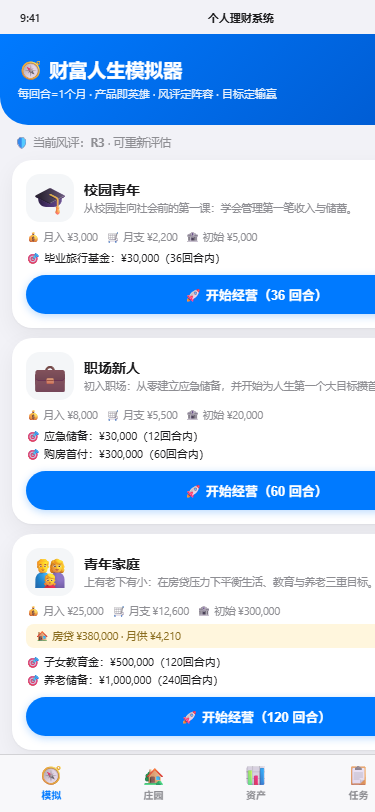
\includegraphics[width=0.23\textwidth]{img/simulator.png}\hfill
  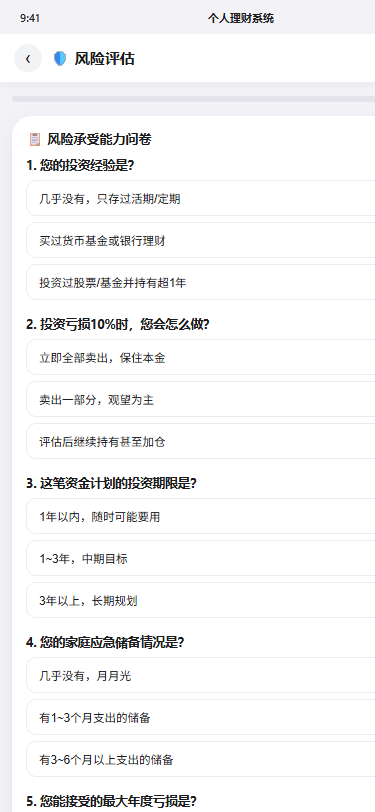
\includegraphics[width=0.23\textwidth]{img/risk.png}\hfill
  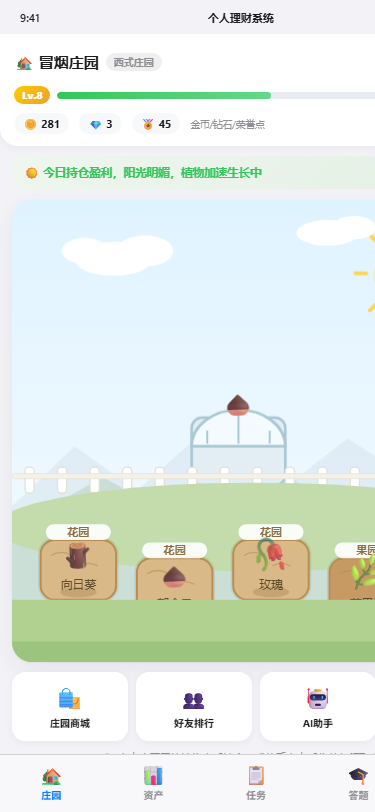
\includegraphics[width=0.23\textwidth]{img/manor.png}\hfill
  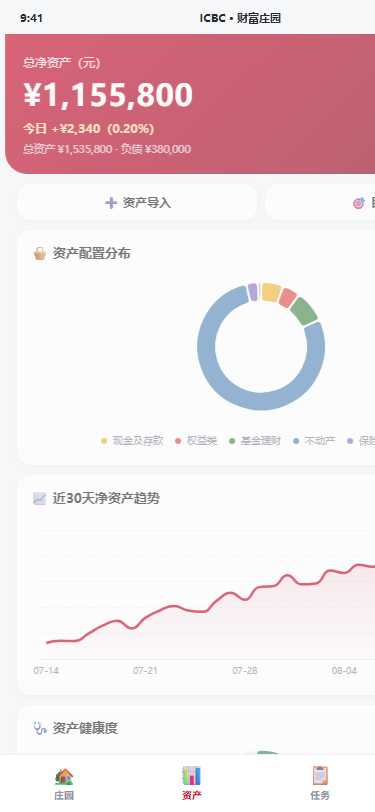
\includegraphics[width=0.23\textwidth]{img/assets.png}
  \\[0.5em]
  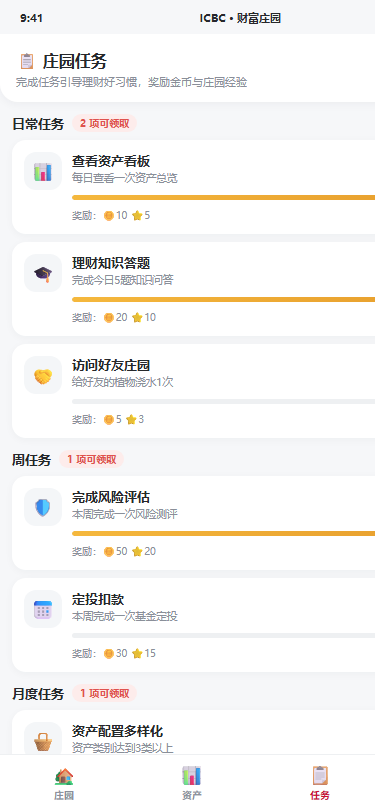
\includegraphics[width=0.23\textwidth]{img/tasks.png}\hfill
  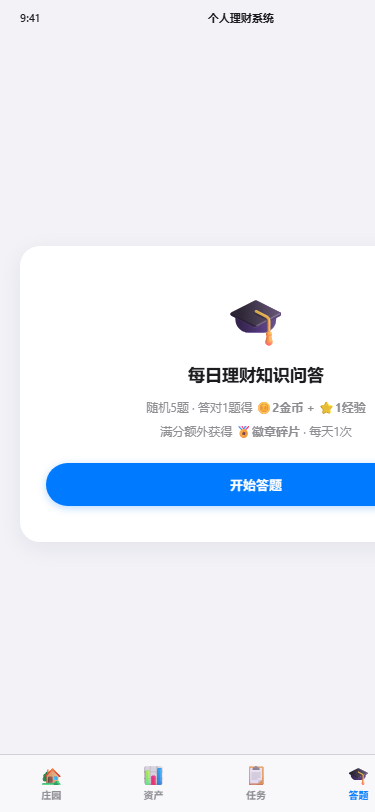
\includegraphics[width=0.23\textwidth]{img/quiz.png}\hfill
  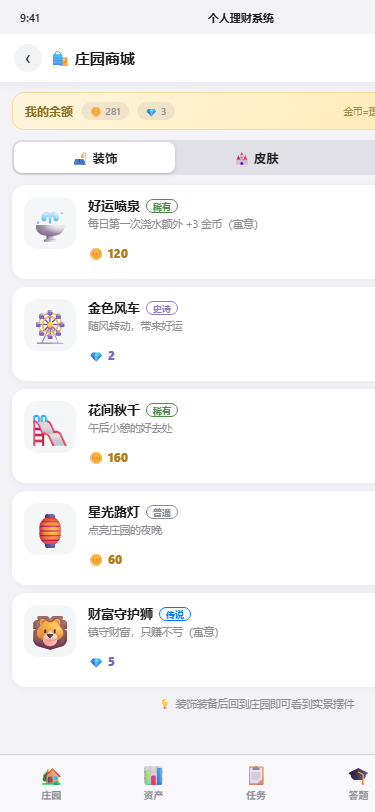
\includegraphics[width=0.23\textwidth]{img/shop.png}\hfill
  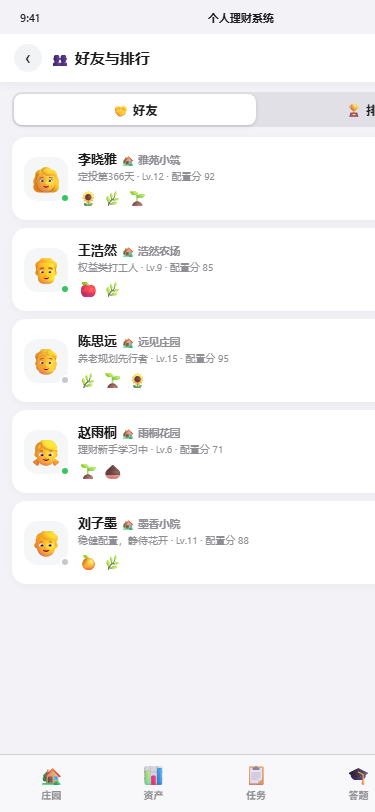
\includegraphics[width=0.23\textwidth]{img/social.png}
  \caption*{图3-1 \quad 个人理财系统演示原型（上排左起：财富人生模拟器、风险评估、财富庄园、资产看板；下排左起：任务中心、知识答题、装扮商城、好友与排行）}
  \end{figure}
}{
  \begin{center}
  \fbox{\parbox{0.82\textwidth}{\centering\vspace{2.5em}
  \large 演示截图占位区\par\vspace{0.8em}
  \small 运行演示原型后，执行 \texttt{wealth-manor/scripts/capture-demo.mjs}
  自动生成截图并重新编译本文档即可插入。\par\vspace{2.5em}}}
  \end{center}
}

\sub{4. 演示环境与后续演进}
原型演示环境为本地浏览器（桌面浏览器以手机框呈现，手机/平板全屏整屏运行，同 WiFi 设备可直接访问）。生产演进路径为：Mock数据层 $\rightarrow$ 对接银行/券商等真实机构账户、产品与行情接口 $\rightarrow$ Cocos Creator 游戏引擎替换SVG场景 $\rightarrow$ 接入行内AI平台与大模型 $\rightarrow$ 独立 App 打包发布与灰度迭代。

% ============================================================
% 四、商业模式（来源：财富庄园C.docx）
% ============================================================
\ch{四、商业模式}

《财富庄园》定位为一款独立开发、独立运营的游戏化财富管理教育产品，采用"B2C用户验证+B2B机构合作"的双轮商业模式。产品前期面向青年用户独立上线，以真实反馈验证趣味性、教育成效和持续使用价值；形成成熟产品及可量化结果后，再通过产品授权、品牌定制、联合运营或私有化部署等方式，优先寻求与工商银行合作。个人用户是直接使用者，工商银行、高校和企业是潜在机构客户。

\sect{（一）目标客户}
\sub{1. 核心用户：18--26岁财富管理起步人群}
核心用户包括高校学生和初入职场青年。该群体具有较强的财富管理意愿，但普遍面临可支配收入有限、金融知识碎片化、风险识别能力不足和理财习惯尚未形成等问题。传统课程专业术语较多，真实投资又存在试错成本，容易降低其持续学习意愿。

《财富庄园》将金融知识内化为游戏规则，使用户在无需投入真实资金的环境中经历收入、消费、储蓄、投资、负债和突发事件，并通过"选择—结果—复盘"的过程理解不同决策的长期影响。

例如，用户在"财富人生棋盘"中可能遇到工资到账、临时医疗支出、信用消费优惠或高收益项目推荐等情境，需要在消费、储蓄、投资和应急资金之间作出选择。系统据此生成"财富偏差护照"，识别冲动消费、从众投资、忽视流动性或风险意识不足等倾向，引导用户理解收益、风险、流动性和生活目标之间的权衡。

\sub{2. 成长用户：27--35岁青年家庭}
该群体收入逐渐稳定并开始承担家庭责任，财富管理需求由基础储蓄转向购房、保险、养老、子女教育和家庭资产配置。针对这类用户，项目将逐步推出家庭财富地图、人生目标规划、应急储备测算和长期现金流模拟，帮助其比较不同人生方案对现金流、风险承受能力和生活目标的影响。

\sub{3. 核心机构客户：工商银行}
工商银行是项目优先争取的机构合作客户。完成独立开发和用户验证后，团队可提供经过市场检验的游戏化金融教育产品，帮助工行丰富青年客户服务形式、增强品牌年轻化形象并提升金融消费者教育效果。工商银行可根据业务需求选择以下引进方式。

\begin{table}[htbp]
\centering
\begin{tabular}{p{3cm}p{4.2cm}p{5.4cm}}
\toprule
\textbf{引进方式} & \textbf{合作内容} & \textbf{适用场景} \\
\midrule
产品授权 & 获得一定期限内的软件使用权 & 青年客户教育、线上主题活动 \\
品牌定制 & 定制工行主题界面、人物形象和专属关卡 & 校园金融节、青年客户活动 \\
联合运营 & 共同策划活动、关卡和推广方案 & 校园推广、金融教育宣传活动 \\
模块采购 & 单独引进反诈、预算或资产配置小游戏 & 工行网点、金融教育专区 \\
私有化部署 & 按照工行数据安全和系统要求独立部署 & 后期大规模正式应用 \\
\bottomrule
\end{tabular}
\caption*{表4-1 \quad 工商银行引进方式}
\end{table}

独立版本不访问工商银行客户账户，主要使用模拟数据或用户自愿录入的非敏感信息。只有在双方正式合作、用户明确授权并满足安全与合规要求后，才考虑连接银行服务接口。该模式可降低工行前期研发和试错成本，使其能够根据验证结果选择引进相应模块。

\sub{4. 其他场景合作客户}
项目还可面向高校和企业提供场景化金融教育服务。高校可借助"校园财富挑战赛"开展金融素养教育；企业可通过定制关卡帮助新员工学习工资规划、社会保险、信用管理和反诈知识，从而形成"青年用户直接使用、工商银行优先引进、高校与企业拓展应用"的多层客户结构。

\begin{table}[htbp]
\centering
\begin{tabular}{p{3cm}p{4.6cm}p{5cm}}
\toprule
\textbf{客户类型} & \textbf{核心需求} & \textbf{项目提供的服务} \\
\midrule
高校学生 & 预算管理、反诈和基础理财 & 财富人生棋盘、反诈闯关、预算小游戏 \\
初入职场青年 & 工资管理、储蓄和风险识别 & 财富偏差护照、目标规划 \\
青年家庭 & 购房、保险和家庭资产配置 & 家庭财富地图、现金流模拟 \\
工商银行 & 青年客户教育、品牌年轻化 & 产品授权、品牌定制、联合运营 \\
\bottomrule
\end{tabular}
\caption*{表4-2 \quad 目标客户与对应服务}
\end{table}

\sect{（二）定价策略}
项目遵循"基础教育免费、进阶服务低价、机构合作为主要收入来源"的原则，不依靠强制广告、充值抽奖或金融产品销售获利，避免商业目标影响金融教育的客观性。

\sub{1. 个人用户定价}
个人用户可免费下载基础版，体验财富人生棋盘、四类理财小游戏、财富庄园和基础行为报告。后期推出的成长版提供更多人生剧本、进阶画像、家庭目标模拟和个性化训练计划。以下价格为试运营建议，后续根据用户付费意愿调整。

\begin{table}[htbp]
\centering
\begin{tabular}{p{3cm}p{5.6cm}p{4cm}}
\toprule
\textbf{产品版本} & \textbf{主要内容} & \textbf{建议价格} \\
\midrule
基础版 & 基础棋盘、四类小游戏、财富庄园 & 免费 \\
成长版 & 更多人生剧本、进阶画像、家庭目标模拟 & 9.9元/月或69元/年 \\
活动主题包 & 校园、职场、青年家庭等主题剧情 & 单独定价或会员免费 \\
\bottomrule
\end{tabular}
\caption*{表4-3 \quad 个人用户版本与建议价格}
\end{table}

个人付费并非项目初期的主要收入来源。低价成长版主要用于验证个性化财富教育需求，同时保证核心金融教育功能对所有用户开放。

\sub{2. 机构客户定价}
工商银行等机构客户采用"年度授权费+定制开发费+运营服务费"的组合定价方式。年度授权费按照使用人数、期限和功能模块确定；定制开发费取决于品牌界面、专属人物、金融内容和部署要求；运营服务费涵盖活动设计、关卡更新、用户反馈分析和阶段性效果报告。

\begin{table}[htbp]
\centering
\begin{tabular}{p{3cm}p{3.6cm}p{6cm}}
\toprule
\textbf{收费项目} & \textbf{收费方式} & \textbf{主要内容} \\
\midrule
软件授权 & 按年或按项目收费 & 使用标准版产品及核心功能 \\
模块采购 & 按功能模块收费 & 单独采购反诈、预算、资产配置等小游戏 \\
品牌定制 & 一次性项目报价 & 定制品牌形象、专属关卡和活动页面 \\
私有化部署 & 根据工作量报价 & 独立部署、安全适配和系统维护 \\
联合运营 & 基础服务费+运营费用 & 活动策划、内容更新和用户分析 \\
高校企业服务 & 按场次或参与人数收费 & 金融课程、团队竞赛和学习报告 \\
\bottomrule
\end{tabular}
\caption*{表4-4 \quad 机构客户收费模式}
\end{table}

项目初期可向工商银行或高校提供小范围试点，以真实数据验证产品效果；试点结束后，再根据活跃用户规模、功能范围和定制深度制定正式报价。

\sub{3. 非交易型奖励机制}
游戏奖励与金融知识进步和健康财富行为相联系，不与投资金额、交易次数或短期收益挂钩。用户可通过反诈训练、连续预算记录、建立应急储备目标和完成资产配置训练获得徽章、庄园装饰或新地图。项目不设置"投入资金越多、升级越快"的机制；若后期由工商银行引进，积分和客户权益方案须由双方共同审核。

% ============================================================
% 五、团队与管理（来源：财富庄园C.docx）
% ============================================================
\ch{五、团队与管理}

\sect{（一）团队概况}
项目团队由三名成员组成，包括两名应用经济学专业学生和一名应用数学专业学生，形成"金融与商业分析—产品与用户研究—数据与技术设计"的跨学科结构。应用经济学成员侧重用户需求、金融行为、商业模式和机构合作；应用数学成员侧重游戏数值、行为评分、数据指标和技术可行性。

团队采用"模块负责+交叉复核+共同决策"的协作机制。每项任务由一名成员主责、另一名成员从不同专业角度复核，降低金融逻辑、用户体验和技术实现相互脱节的风险。

\sect{（二）职能分工}
\begin{table}[htbp]
\centering
\begin{tabular}{p{2.2cm}p{2.6cm}p{3.2cm}p{4.6cm}}
\toprule
\textbf{团队成员} & \textbf{专业背景} & \textbf{团队角色} & \textbf{主要职责} \\
\midrule
王思佳 & 应用经济学 & 项目与商业负责人 & 项目统筹、商业模式、机构合作、战略规划、进度管理和企划书整合 \\
阮馨莹 & 应用经济学 & 产品与金融内容负责人 & 用户研究、市场分析、金融场景与关卡设计、合规边界检查 \\
张煜杰 & 应用数学 & 数据与技术负责人 & 游戏数值、财富行为评分、数据指标、技术架构和原型可行性分析 \\
三人共同 & 跨专业协作 & 核心决策小组 & 共同确定产品定位、核心玩法、创新点、原型迭代和答辩方案 \\
\bottomrule
\end{tabular}
\caption*{表5-1 \quad 团队成员职能分工}
\end{table}

团队以两周为一个工作周期，每周召开一次进度会议，明确任务、负责人、交付成果和时间节点；周期结束后进行内部评审，并根据完成情况和用户反馈调整计划。项目文档实行统一版本管理，确保产品名称、目标用户、游戏规则、商业模式和数据指标口径一致。

出现意见分歧时，团队按照"是否回应真实需求、是否符合金融安全要求、是否具备现实可行性"三个标准判断，必要时通过用户调查或原型测试作出决策。

% ============================================================
% 六、项目规划（来源：财富庄园C.docx；技术创新战略为新撰写）
% ============================================================
\ch{六、项目规划}

\sect{（一）总体战略}
《财富庄园》采用"独立开发—用户验证—产品迭代—机构引进"的总体战略。项目先在不依赖工商银行系统、客户数据和开发资源的前提下完成原型及真实用户测试；验证趣味性、教育成效和持续使用价值后，再以完整原型、测试结果和合作方案争取产品授权、联合运营或定制部署。

"一核"：以提升青年用户的财富决策能力为核心，不以短期模拟收益作为唯一标准，而是关注预算意识、风险意识、长期规划和独立判断能力。

"双端"：个人用户端负责验证产品是否好玩、易懂、有效；机构客户端面向工商银行、高校和企业提供可引进、可定制、可持续运营的金融教育方案。

"三步走"：依次完成产品验证、市场验证和机构合作，以真实用户数据降低机构引进的不确定性。

产品由三层游戏结构构成：第一层"财富人生棋盘"模拟升学、就业、消费、租房、投资和突发事件；第二层3--5分钟专项小游戏训练预算、反诈、资产配置和投资情绪管理；第三层"财富庄园"将学习成果、行为变化和财富规划转化为长期可视化成长。金融知识由此不再是附加题库，而成为推动游戏决策的核心规则。

\sect{（二）战略规划与实施}
项目计划用24周完成从需求验证到机构试点准备的全过程。

\lead{1. 第一阶段：需求验证与产品定位（第1--4周）。}{通过不少于100份有效问卷及针对高校学生、初入职场青年的访谈，识别其在消费、储蓄、投资和金融学习方面的困难，确定核心用户画像、首批游戏场景和商业模式，形成需求报告、游戏规则初稿及低保真原型。}
\lead{2. 第二阶段：独立产品原型开发（第5--12周）。}{围绕"随机事件—财富选择—资产变化—结果反馈—对比复盘—庄园成长"的完整闭环，开发财富人生棋盘、财富庄园以及预算管理、金融反诈、资产配置和投资情绪四类小游戏；同步形成"财富偏差护照"。独立版本仅使用模拟数据或用户自愿录入的信息，不接入真实银行账户。}
\lead{3. 第三阶段：用户测试与市场验证（第13--18周）。}{在高校学生和青年用户中开展小范围测试，重点检验规则理解度、持续吸引力、知识提升和行为报告的实用性。阶段性目标为核心关卡完成率不低于70\%、单局时长控制在3--5分钟、测试后金融知识正确率较测试前提升20\%。团队据此优化难度、奖励、界面、剧情和复盘机制。}
\lead{4. 第四阶段：机构试点与商业合作（第19--24周）。}{完成用户验证后，制作面向工商银行的产品引进方案，包括产品介绍、模块清单、测试结果、品牌定制、合作模式、数据安全和初步成本测算。试点优先采用独立演示、活动版或品牌定制版，不直接接入银行核心业务系统；达到预期后，再讨论软件授权、联合运营或私有化部署。}

\begin{table}[htbp]
\centering
\begin{tabular}{p{2.6cm}p{2cm}p{4.6cm}p{3.4cm}}
\toprule
\textbf{阶段} & \textbf{时间} & \textbf{核心任务} & \textbf{主要成果} \\
\midrule
需求验证 & 第1--4周 & 问卷、访谈、用户画像及玩法确认 & 需求报告、游戏规则、低保真原型 \\
产品开发 & 第5--12周 & 开发人生棋盘、小游戏和庄园系统 & 可交互原型、财富偏差护照 \\
市场验证 & 第13--18周 & 用户测试、数据分析及产品迭代 & 测试报告、优化版独立产品 \\
机构合作 & 第19--24周 & 制作引进方案、争取工行试点 & 产品演示、合作方案、试点计划 \\
\bottomrule
\end{tabular}
\caption*{表6-1 \quad 项目实施路线图}
\end{table}

项目评价从趣味性、教育性、行为改善、产品可持续性和机构引进价值五个维度展开，分别考察关卡完成与留存、知识提升、预算储蓄与风险意识、使用及付费意愿，以及定制能力、部署灵活性和金融教育效果。

\sect{（三）技术创新战略}
项目以"金融级严谨、游戏化体验、数据驱动迭代"为技术主线，已交付可运行的独立演示原型（Vue 3 + Express 全栈，前后端分离，RESTful 规范），并规划以下技术创新路径：

\lead{1. 模拟器引擎——纯函数状态机。}{财富人生模拟器的核心引擎采用纯函数设计：风险评估评分、产品资格判定、经济周期×政策收益率状态机、回合推进（发薪—事件—决策—结算）、目标校验与财富偏差护照均为无副作用纯函数，可独立单元测试（26例全过）与确定性复现（固定种子事件队列），保障金融逻辑严谨可审计。}
\lead{2. 五层服务架构与工程化实现。}{生产环境采用"客户端—网关—BFF聚合—微服务—数据层"五层架构，演示原型以"路由 $\rightarrow$ 服务 $\rightarrow$ Provider $\rightarrow$ 数据"四层结构一一对应，接口版本化（\texttt{/api/v1}）、统一响应规范（\texttt{\{code, message, data\}}），保证从原型到生产的平滑演进。}
\lead{2. 轻量游戏引擎方案。}{游戏场景采用 Cocos Creator 3.x 渲染（包体增量约8MB），支持 H5 与原生混合渲染、独立 App 与内嵌双形态发布；演示原型以 SVG 手绘风实现同构交互接口，可无损替换。}
\lead{3. AI 双引擎决策支持。}{采用"大模型生成 + 规则引擎兜底"双引擎：大模型负责对话式问答与生成式建议，规则引擎保证建议可解释、可审计、合规可控；当前演示版已实现数据驱动的规则问答与资产健康度评分、配置建议、目标测算等能力。}
\lead{4. 数据驱动设计。}{植物物种、任务定义、知识题库、商城商品、AI 问答规则均为纯配置数据，新增内容无需改动代码；趋势模拟采用确定性随机种子，保证演示与回归测试可复现。}
\lead{5. Provider 注册表抽象。}{数据访问通过 Provider 注册表统一路由，Mock 与真实机构数据源实现同契约切换（\texttt{DATA\_PROVIDER} 环境变量），对接银行/券商账户、行情、OCR 等外部服务时业务层零改动。}
\lead{6. 金融级安全与体验差异化。}{国密 SM2/SM4 + TLS 1.3 全链路加密、资产数据仅展示不落库、本地 OCR 优先、游戏时长每日30分钟防沉迷上限；界面采用 Apple 设计语言（iOS 蓝色系色板、毛玻璃、连续圆角体系）并适配手机/平板/桌面多端分辨率，形成技术与体验双重的产品壁垒。}

\sect{（四）人才战略}
项目采用"竞赛核心团队+专业协作人才池"的人才模式。竞赛及原型阶段由现有三人团队完成用户研究、产品设计、商业模式、游戏机制、数据方案和原型制作；进入实际开发与机构合作阶段后，再根据需要引入UI/UX设计、游戏开发、金融产品、消费者权益保护、数据安全、测试运营和商务合作人员。

金融与消费者权益保护人员负责审核关卡内容和风险提示；技术与数据安全人员保障产品稳定运行和个人信息安全；商务人员负责机构授权、定制和试点沟通。团队拟邀请校内相关专业教师提供阶段性指导，并争取工商银行专业人员提出建议；在正式合作前，不将外部人员或工商银行表述为现有团队成员或已确定合作方。

\sect{（五）项目进展}
截至2026年8月，项目处于"产品方案基本形成、独立原型准备验证"阶段。

\textbf{已完成}：参赛方向、目标用户、核心痛点和独立产品定位已经明确；"财富人生棋盘+专项理财小游戏+财富庄园"的三层结构以及随机事件、财富树、知识任务、财富行为画像等核心机制已形成初步方案。同时，团队已完成"个人理财系统"独立演示原型的开发——覆盖登录、新手引导、财富庄园（种植/天气/收获闭环）、资产看板（配置/趋势/健康度/AI建议/财富树）、任务中心、知识答题、装扮商城、好友排行、AI助手、目标规划、资产导入与个人中心全量核心模块，并通过单元测试与接口冒烟测试验证（详见"三、产品与服务"之平台演示）。

\textbf{正在推进}：团队正在完善商业模式、游戏规则、数值体系、技术架构和可交互原型。目前尚未与工商银行达成正式合作，也未接入其客户数据或业务系统；工商银行是项目优先争取的潜在机构客户。

\textbf{下一阶段}：优先完成"事件出现—用户选择—结果变化—对比复盘—庄园成长"的核心闭环并开展青年用户测试，再以真实测试结果形成面向工商银行的引进方案，提高商业合作的可信度和落地可能性。

\end{document}
